\chapter{Россби}
В этом разделе мы попробуем осознать сразу несколько крайне важных понятий в метеорологии и океанологии: число Россби, радиус деформации Россби и волны Россби. 

Все эти термины ввел в геофизику американский метеоролог шведского происхождения Карл Густав Арвид Россби (рис. \ref{fig:A_R1}). Этот ученый, среди прочего, первым предложил использовать уравнения гидродинамики для описания атмосферных движений.  

    \begin{figure}
    \centering
    \begin{minipage}[b]{.5\textwidth} % left
    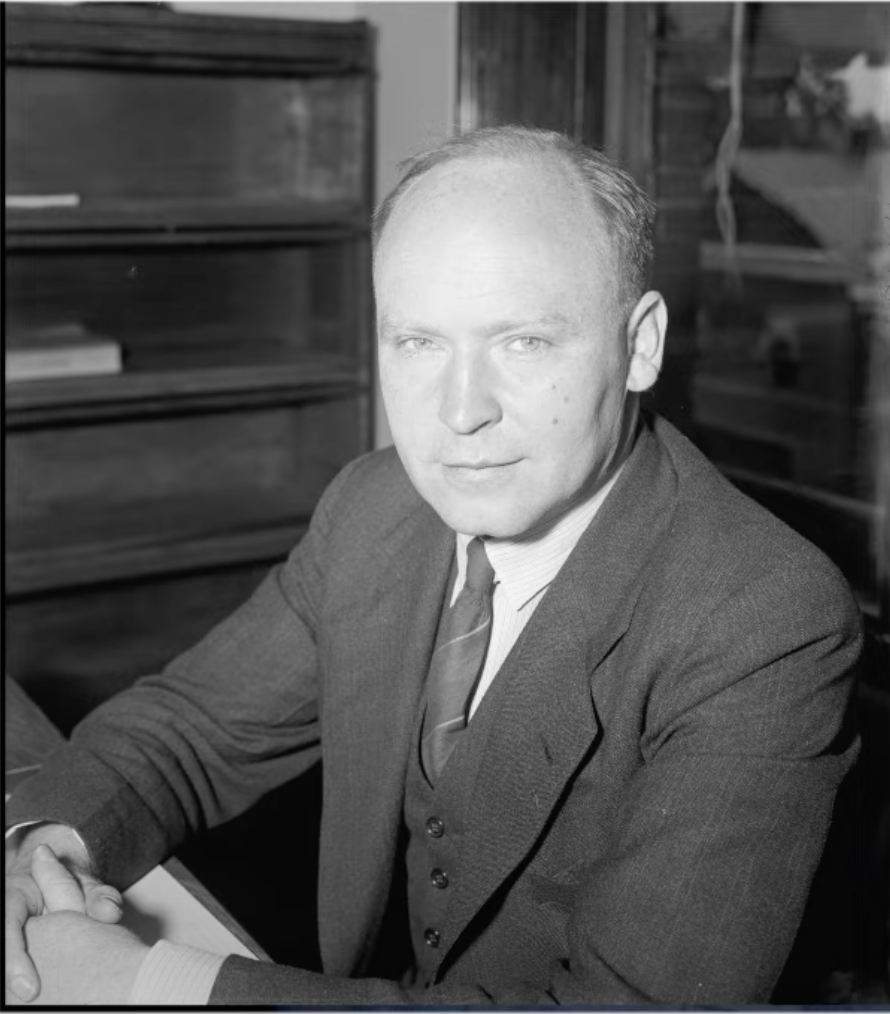
\includegraphics[width=1\linewidth]{pics/A_R1.png}
    \end{minipage}%
    \begin{minipage}[b]{.5\textwidth} % right
      \centering
      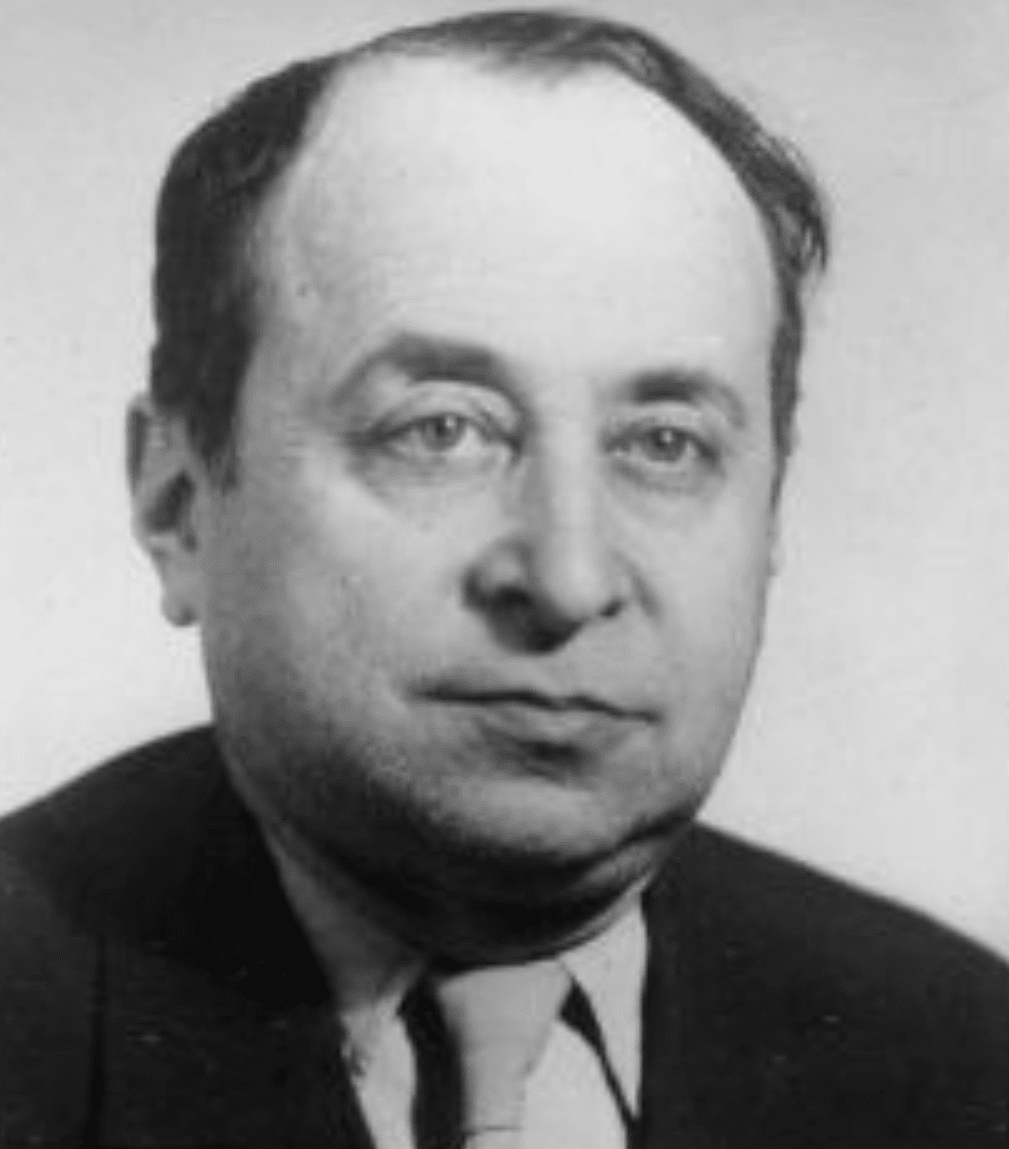
\includegraphics[width=1\linewidth]{pics/A_R2.png}
    \end{minipage}
    \caption{\label{fig:A_R1} Карл Густав Арвид Россби (1898--1957) и Илья Афанасьевич Кибель (1904--1970)}
    \end{figure}

\section{Число Россби} \label{A_Rossby}

Кибель-Россби. Илья Афанасьевич Кибель (1904--1970)

\begin{equation}
    \label{eq:A_Rossby}
    Ro = \frac{\td{u}{t}}{fu} = 
        \frac{ \frac{U}{T} }{fU} = 
        \bigg| \:\: U=\frac{L}{T} \:\: \bigg| = 
        \frac{ \frac{U^2}{L} }{fU} = 
        \frac{U}{Lf}
\end{equation}

% https://youtu.be/aRnZd0UVeDo (можно вщять как визуализацию)
Это отношение сил инерции к силе Кориолиса. Т.е. помогает определить какие силы наиболее важны в данном случае, а какими можно пренебречь. То есть связано с масштабом движения. 

$Ro >> 1$ означает, что превалируют силы инерции и центробежное ускорение ($U>>Lf$). Такие движения как правило малого масштаба, например, торнадо. Малое значение числа Россби $Ro << 1$ характерно для синоптического масштаба (циклоны).

% https://youtu.be/xOip9XlsoDU?si=EElC8jOstldUCrHu
С точки зрения силы Кориолиса: если движения малого масштаба $L$, но с большими скоростями $U$, то сила Кориолиса не имеет значения. Но сила Кориолиса играет существенную роль для больших и медленных циркуляций.  
На этому курсе мы рассматриваем синоптические движения, поэтому наша область интересов лежит в диапазоне $R_o >> 1$.

\section{Волны Россби} \label{A_Rossby}

Планетарный масштаб.

% https://youtu.be/VSNllMdW84w
Различают 2 категории: океанические и атмосферные ВР. Океанические ВР упаковываются в термоклин (между теплыми, у поверхности, и холодными в толще океана, водами). Двигаются с востока на запад. 

% https://youtu.be/nwyd5_8eIMM?si=TiD3EdtCoQll062_
% Очень крутой видос про океанические ВР

Атмосферные ВР пакуются (волновод) в средних широтах на высоте верхней тропосферы (струйные течения) и направлены на восток (западный перенос). Если скорость потока замедляется, то возникает эффект <<блокинга>>, когда поле давление оказывается запертым над какой-то территорией. Это приводит к пожарам в области высокого давления и наводнениям в области низкого давления. 

Атмосферные ВР бывают синоптические (вызванные атмосферными процессами, как правило быстрые) и вынужденные (искривление за счет препятствий планетарного масштаба)

% https://youtu.be/KTpvIzCdHvg?si=beKX_c_L3oyrTcPz 
В атмосферных ВР $Ro \sim 1$. Размер волны бывает короткий (100-1000 км) этот тип быстро перемещается и длинный (2000+ км) -- это уже планетарные волны. Как правило короткие волны модулируются на длинных. Иногда короткие волны толкают блокирующую ситуацию длинных волн. 

% Нолтон pp 97-99 eq (4.13)
Как образуются волны Россби. Нарисовать им на доске. 

\section{Радиус деформации Россби} \label{A_Rossby}
В метеорологии и океанологии радиус деформации Россби это масштаб длины на котором эффекты вращения становятся такими же важными, как и эффекты плавучести (Гилл, 1986)
% Гилл А. Динамика атмосферы и океана: в 2-х томах. Т. 2. М.: Мир, 1986. 415 с.
% https://www.researchgate.net/publication/344174324_Metody_ocenki_baroklinnogo_radiusa_deformacii_Rossbi

Для баротропной среды радиус деформации представлен как 
\begin{equation}
    L_R = \frac{{gD}^{1/2}}{f},
\end{equation}
где $g$ -- ускорение свободного падения, $D$ -- глубина слоя (воды), а $f$ - параметр Кориолиса. К примеру для широты 45$\deg$ параметр Кориолиса будет $f=10^{-4} \: s^{-1}$, $g=9.8 m/s^2$ радиус деформации Россби будет $L_R\approx2000 km$. Если изменим только глубину $D=40 m$, то $L_R = 200 km$.

В бароклинной среде радиус деформации Россби определяется как 

\begin{equation}
    L_{R,n} = \frac{NH}{n \pi f_0},
\end{equation}
где $N$ - частота Вяйсяля-Брента, $H$ - масштаб высоты, а $n=1,2,...$. Для атмосферы Земли, отношение $N/f_0=100$, таким образом радиус деформации Россби в 100 раз больше вертикального масштаба. Для ситуаций, когда за $H$ взята высота тропопаузы $L_{R,n} \approx 1000 $лм, что соответствует синоптическому масштабу.  

И в атмосфере и в океане размер вихря уменьшается к высоким широтам.